\documentclass{beamer}
\usetheme{CambridgeUS}
\usecolortheme{beaver}

\makeatletter
\defbeamertemplate*{title page}{mydefault}[1][]
{
	\vbox{}
	\vfill
	\begin{centering}

%{\usebeamercolor[fg]{titlegraphic}\inserttitlegraphic\par}
		\begin{beamercolorbox}{titlegraphic}
				\usebeamerfont{titlegraphic}\inserttitlegraphic
		\end{beamercolorbox}%
			\vskip1em\par	
		\begin{beamercolorbox}[rounded=true, center, shadow=true, sep=8pt,#1]{title}
			\usebeamerfont{title}\inserttitle\par%
			\ifx\insertsubtitle\@empty%
			\else%
			\vskip0.5em%
			{\usebeamerfont{subtitle}\usebeamercolor[fg]{subtitle}\insertsubtitle\par}%
			\fi%     
		\end{beamercolorbox}%
		\vskip1em\par
		\begin{beamercolorbox}[sep=8pt,center,#1]{author}
			\usebeamerfont{author}\insertauthor
		\end{beamercolorbox}
		\begin{beamercolorbox}[sep=8pt,center,#1]{institute}
			\usebeamerfont{institute}\insertinstitute
		\end{beamercolorbox}
		\begin{beamercolorbox}[sep=8pt,center,#1]{date}
			\usebeamerfont{date}\insertdate
		\end{beamercolorbox}\vskip0.5em
		\begin{beamercolorbox}[sep=8pt,center,#1]{logo}
			\usebeamerfont{titlegraphic}\insertlogo
		\end{beamercolorbox}%
	\end{centering}
	\vfill
}
\setbeamertemplate{title page}[mydefault]
\makeatother



\titlegraphic{
\includegraphics[width=50mm]{logo_dauphine} \hspace*{5.5cm} 
\includegraphics[width=7mm]{cnrs}}
\title[Elicitation and Explanation in Social Choice]{Elicitation and Explanation in Social Choice Theory}
%\subtitle{Proposal: ``Elicitation and Explanation for Voting Rules''}
\author[Beatrice Napolitano]{\textbf{Beatrice Napolitano} \\
	Supervisors: Remzi Sanver, Olivier Cailloux}
\date[CST 16 May 2019]{Suivi de Thèse \\ 16 May 2019 \\ 
\includegraphics[width=35mm]{LOGO_LAMSADE} }

\usepackage{tikz}
\usepackage{amsmath}
\usepackage{graphicx}
\newcommand{\ppref}{\succ^\text{p}}

\definecolor{darkred}{rgb}{0.8,0,0}

\begin{document}

\beamertemplatenavigationsymbolsempty

\begin{frame}[plain]
\maketitle
\end{frame}

\addtocounter{framenumber}{-1}


\section{Ph.D. Proposal}
\subsection*{Goal}
\begin{frame}
\frametitle{\textbf{Ph.D. Proposal:} Goal}
Develop procedures able to help a committee (or a society) choose a suitable voting rule
\newline \newline \textbf{Involves}:
\begin{itemize}
	\item Axiomatic analysis of voting rules
	\item Explanation of axioms in non-expert terms
	\item Preference elicitation methods
\end{itemize}
\end{frame}

\subsection*{Approach}
\begin{frame}
	\frametitle{\textbf{Ph.D. Proposal:} Approach}
	\textbf{Idea}: Automatically find properties which are incompatible  \newline \newline
	The inconsistencies proofs should be translated to non-expert terms and used for:
	\begin{itemize}
		\item querying the user and infer her preferences depending on her answers
		\item showing the user that she cannot have everything
		\item validate whether some choices are ``better'' than others
	\end{itemize}~\\	
	\textbf{More generally}: Work on elicitation procedures related to social choice
\end{frame}

\section{Current Work}
\subsection{Minimax Regret}

\begin{frame}
\frametitle{\textbf{Current Work:} Simultaneous Elicitation of Committee and Voters Preferences}
%\framesubtitle{Robust Winner Determination}
%	\textbf{Setting}: Two kind of players
\textbf{Setting}: Incomplete profile and uncertain scoring rule
\begin{figure}
	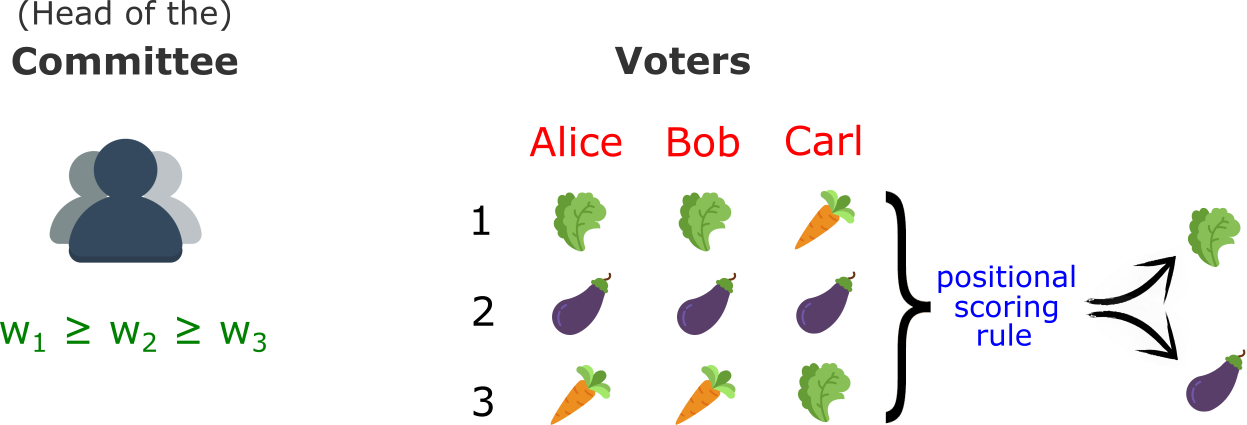
\includegraphics[scale=0.35]{set.png}
	%		\caption{.}
	%		\label{fig:b1}
\end{figure}
\textbf{Goal}: Winner determination using an incremental elicitation protocol based on minimax regret 
\end{frame}
\addtocounter{framenumber}{-1}
\begin{frame}
	\frametitle{\textbf{Current Work:} Simultaneous Elicitation of Committee and Voters Preferences}
	\textbf{Setting}: Incomplete profile and uncertain scoring rule
	\begin{figure}
		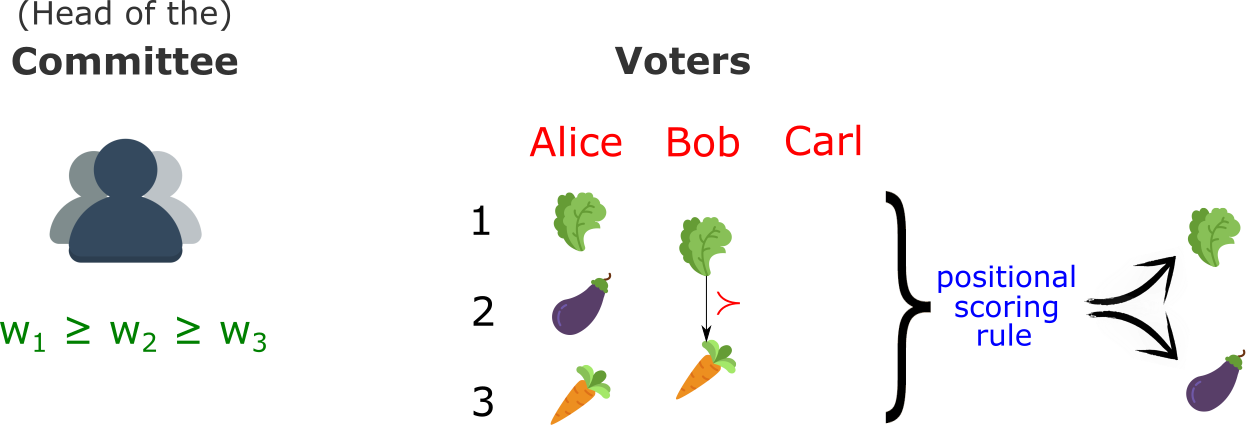
\includegraphics[scale=0.35]{set2.png}
%		\caption{.}
%		\label{fig:b1}
	\end{figure}
	\textbf{Goal}: Winner determination using an incremental elicitation protocol based on minimax regret 
\end{frame}

\subsection{Related Works}
\begin{frame}
	\frametitle{\textbf{Current Work:} Related Works}
	\textbf{Incomplete profile}  
	\begin{itemize}
		\item and known weights: Minimax regret to produce a robust winner approximation (\textit{Lu and Boutilier 2011}, \cite{Lu2011}; \textit{Boutilier et al. 2006}, \cite{Boutilier2006})
	\end{itemize}~\\
	\textbf{Uncertain weights} 
	\begin{itemize}
		\item and complete profile: dominance relations derived to eliminate alternatives always less preferred than others (\textit{Stein et al. 1994}, \cite{Stein1994})
		\item in positional scoring rules (\textit{Viappiani 2018}, \cite{Viappiani2018})
	\end{itemize}
\end{frame}

\section{Submissions}
\subsection{Conferences, Workshops and Summer Schools}
\begin{frame}
	\frametitle{Conferences, Workshops and Summer Schools}
	\textbf{Conferences}  
	\begin{itemize}
		\item Short paper regarding the work conducted with Olivier Cailloux and Paolo Viappiani accepted to RJCIA 2019 (Toulouse 1-5 July)
		\item Deliberation, Belief Aggregation, and Epistemic Democracy II (Neuville-sur-Oise 11-13 June)
	\end{itemize}~\\
	\textbf{Workshops} 
	\begin{itemize}
		\item Poster submission to 3rd ILLC Workshop on Collective Decision Making (Amsterdam 6-7 June)
	\end{itemize}~\\
	\textbf{Summer Schools}  
	\begin{itemize}
		\item International Summer School "Preferences, decisions and games" (Paris 25-28 June) and presentation of the current work
	\end{itemize}
\end{frame}

\section{Academic Life}
\begin{frame}
	\frametitle{Academic Life}
	\textbf{Courses Attended}  
	\begin{itemize}
		\item \textbf{Market Design} - prof. Sidartha Gordon, Oct-Nov 2018
		\item \textbf{Probabilistic Methods} - prof. Ararat Harutyunyan, Mar-May 2019
	\end{itemize}~\\
	\textbf{Supervisors} 
	\begin{itemize}
		\item Awesome people, always available and helpful
		\item Perfect guides
		\item Weekly meetings
	\end{itemize}~\\
	\textbf{Office}  
	\begin{itemize}
		\item Great relationships with all the other Ph.D. students
		\item Friendly and funny vibes in the lab
	\end{itemize}
\end{frame}

\section{Goals}
\begin{frame}
	\frametitle{Goals} 
	\begin{itemize}
		\item Submit the current work in at least one big conference in Fall 2019
		\item Carry on a parallel work about the concept of compromise in bargaining 
		\item Become fluent in French and teach from January 2020
		\item Visit the Louvre 
	\end{itemize}
\end{frame}

\addtocounter{framenumber}{-1}
\begin{frame}[plain]
	\centering \color{darkred}\LARGE Thank You!
\end{frame}




\bibliographystyle{plain}
\bibliography{biblio} 
%given a combination of axioms we want to find an outcome that doesn't satisfy them, and we would do that for several reasons:
%-querying the user, depending of her answer we might infer her preferences over the set of axioms;
%-proving that a set of axioms is not valid giving a counter-example;


%A method for automatically proving impossibility theorems in the area of ranking sets of objects has already been implemented (Geist \& Endriss, 2011). It:



\end{document}